%!TEX program = xelatex

%% 版本：1.0
%% 2024-07-02
%% 原作者：景宗雷
%% 燕山大学适配：Codex
\documentclass[aspectratio=169,UTF8,t]{beamer}%比例是16:9，UTF8编码支持，顶部对齐
\usepackage{ysuslide}
\usepackage[UTF8]{ctex}
\usepackage{xeCJK}
\usepackage{fontawesome}%加入图标支持
\usepackage{tcolorbox}
\usepackage{verbatim}
\usepackage{caption}
\usepackage{subcaption}

\newcommand\crule[3][black]{\textcolor{#1}{\rule{#2}{#3}}}

%基本信息
\title{燕山大学幻灯片 LaTeX 模板}
\subtitle{厚德、博学、求是}
\author{作者姓名}
\date{\today}
\institute{学院名称}
\newcommand{\last}{敬请批评指正！} %结束语
%\newcommand{\last}{提问与解答环节}
%基本信息结束

\begin{document}

\maketitle

\makeoutline

\section{简介}

\subsection{模板简介}

\begin{frame}
    \frametitle{简介}
    燕山大学演示文稿 LaTeX 非官方模板。

    本模板修改自 ouc-slide-latex-template\footnote{https://github.com/dryangyq/ouc-slide-latex-template} 模板，并进行了燕山大学适配。

    模板主要使用燕山大学形象识别系统\footnote{https://vis.ysu.edu.cn/}，包括燕大蓝、亮蓝色、浅蓝色、辅助红、中性灰、金色、银色。

    此外，使用了大量的信息框来增加模板的活力。
    \begin{center}
        \begin{figure}
        \centering
        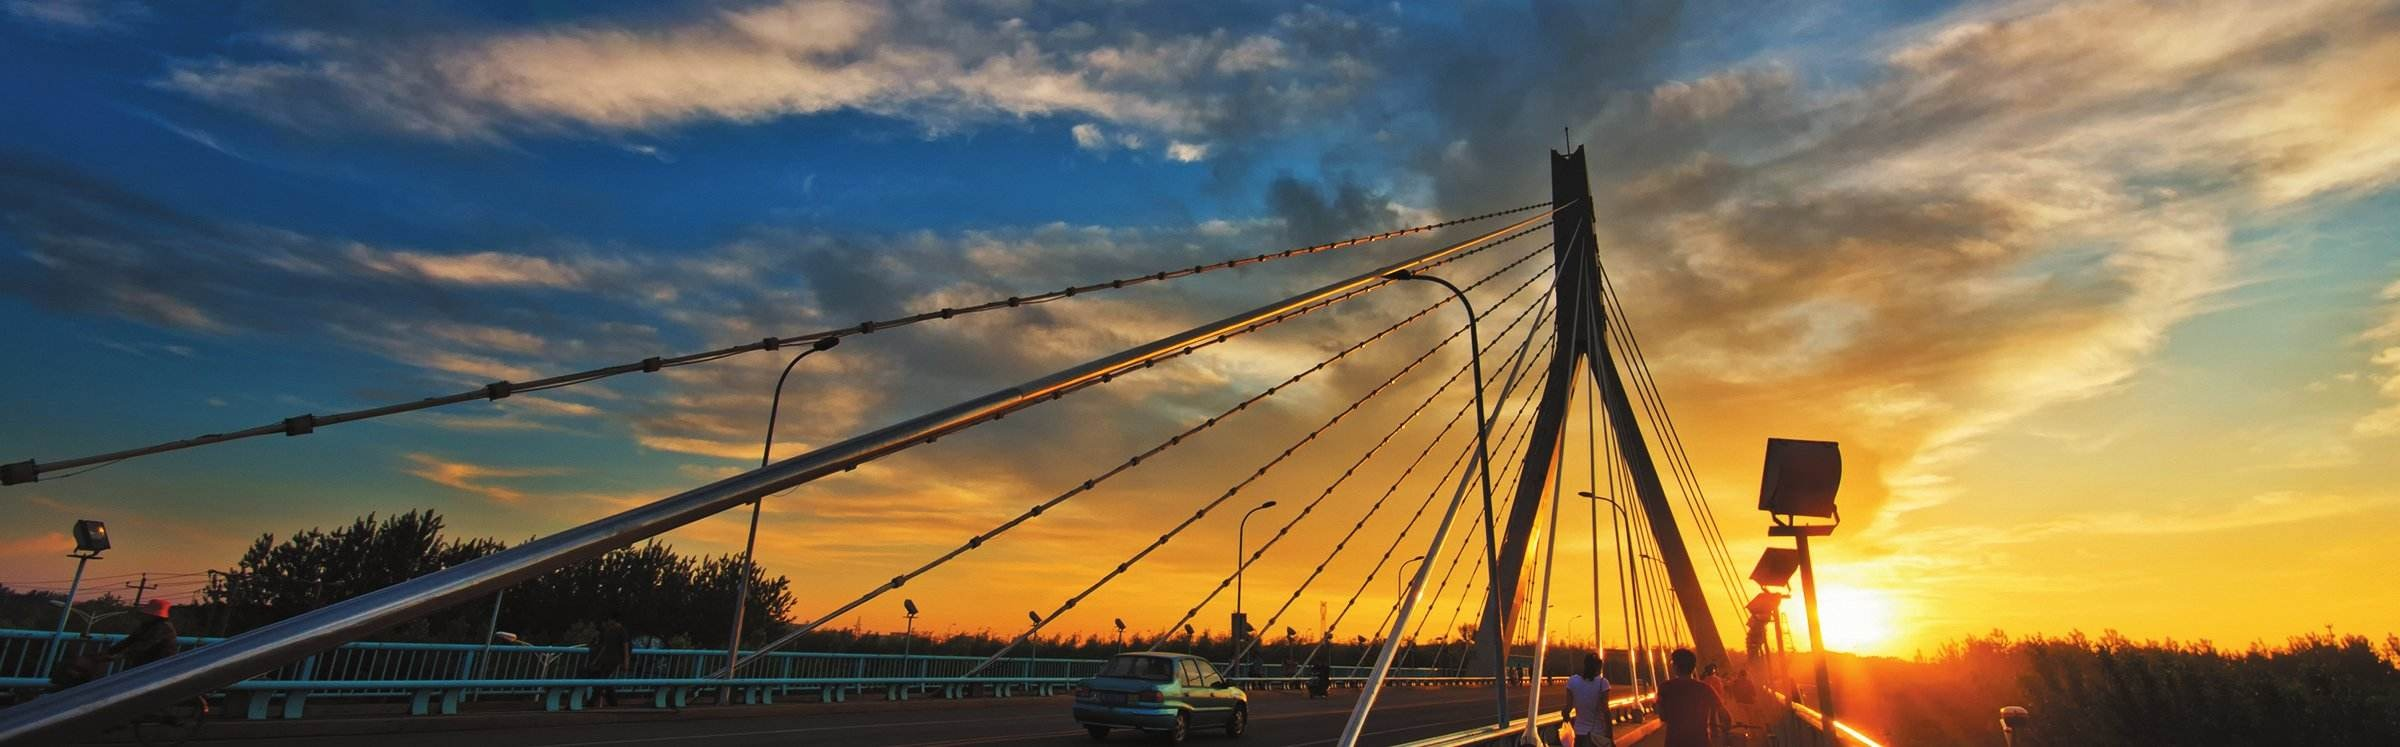
\includegraphics[width=0.56\textwidth]{figs/ysu_campus.jpg}
            \caption{燕山大学校园景观}
            \label{fig:main}
        \end{figure}
    \end{center}
    
    
\end{frame}

\section{模板使用方法}

\subsection{使用方法}

\begin{frame}
    \frametitle{模板使用方法}    
    \begin{enumerate}
        \item 从 git 上 clone 整个项目目录\\~
        \item 编辑tex文件进行修改\\~
        \item 编译tex文件为PDF\\~
        \begin{enumerate}
            \item 可以使用VS Code，或者\\~
            \item 使用LaTeX IDE，比如TeXstudio等进行编译\\~
        \end{enumerate}
        \item \emph{注意：} 请使用LuaLaTeX 或者 XeLaTeX 进行编译
    \end{enumerate}
\end{frame}

\section{元素}

\subsection{字体}

\begin{frame}
    \frametitle{字体是啥}
    模板参考燕山大学 VIS 手册中的方正黑体、Helvetica 等专用印刷字体规范。
    默认使用随模板分发的 HarmonyOS Sans，保证屏幕展示清晰、跨平台编译一致。

    如需严格按纸质印刷规范制作，可将方正兰亭黑、方正细黑等字体放入 fonts 文件夹，
    并在\textbf{beamerfontthemeYSUSlide.sty}中修改。
    \begin{center}
        \begin{figure}
        \centering
        \includegraphics[width=0.44\textwidth]{figs/harmonysans.png}
            \caption{鸿蒙字体}
            \label{fig:harmonysans}
        \end{figure}
    \end{center}
\end{frame}

\subsection{颜色}
\subsubsection{基本颜色}
\begin{frame}
    \frametitle{颜色}
    %\framesubtitle{基本颜色}
    
    根据燕山大学形象识别系统，定义了相关颜色，主要包括燕大蓝、亮蓝色、浅蓝色、辅助红、中性灰、金色、银色。其中文名称和代码如表\ref{table:color}所示。\\
    当然，也可以使用Latex自带的颜色，例如white、black等。
    
    \begin{table}
        \centering
        \small
        \caption{基本颜色定义}
        \label{table:color}
        \begin{tabular}{ccc}
            \textbf{颜色} & \textbf{名称} & \textbf{中文名}\\\toprule
            \crule[ysublue]{10pt}{10pt} & ysublue & 燕大蓝 \\
            \crule[ysubrightblue]{10pt}{10pt} & ysubrightblue & 亮蓝色 \\
            \crule[ysulightblue]{10pt}{10pt} & ysulightblue & 浅蓝色 \\
            \crule[ysured]{10pt}{10pt} & ysured & 辅助红 \\
            \crule[ysugray]{10pt}{10pt} & ysugray & 中性灰 \\
            \crule[ysugold]{10pt}{10pt} & ysugold & 金色 \\
            \crule[ysusilver]{10pt}{10pt} & ysusilver & 银色 \\
        \end{tabular}
    \end{table}
\end{frame}

\subsubsection{颜色等级}

\begin{frame}
    \frametitle{颜色}
    %\framesubtitle{颜色等级}
    
    \emph{定义的燕山大学标准色，每一种颜色，都有九个等级，等级越低，颜色越浅。例如：对于燕大蓝，其等级颜色如表\ref{table:colorgrade}所示。}\\
    
    \begin{table}
        \centering
        \small
        \caption{颜色等级}
        \label{table:colorgrade}
        \begin{tabular}{cl}
            \textbf{颜色} & \textbf{名称}\\\toprule
            \crule[ysublue20]{8pt}{8pt} & ysublue20 \\
            \crule[ysublue30]{8pt}{8pt} & ysublue30 \\
            \crule[ysublue40]{8pt}{8pt} & ysublue40 \\
            \crule[ysublue50]{8pt}{8pt} & ysublue50 \\
            \crule[ysublue60]{8pt}{8pt} & ysublue60 \\
            \crule[ysublue70]{8pt}{8pt} & ysublue70 \\
            \crule[ysublue80]{8pt}{8pt} & ysublue80 \\
            \crule[ysublue90]{8pt}{8pt} & ysublue90 \\
            \crule[ysublue]{8pt}{8pt} & ysublue \\\bottomrule
        \end{tabular}
    \end{table}
\end{frame}

\subsection{副标题和列表}

\subsubsection{\textbf{副标题}：可以补充更多信息}

\begin{frame}
    \frametitle{副标题和列表}
    副标题，可以展示不同的层级关系，一般用来显示内部章节。\\
    幻灯片的标题，都使用section进行规划，内部的frametitle中的内容将不再起作用。一级标题，使用单独的幻灯片进行展示，并显示在目录幻灯片中。二级和三级标题，在幻灯片的标题部分进行显示，带有自动编号。\\
    可以使用内部列表展示幻灯片中的层级关系。这里是无序列表的样子。
    \begin{itemize}
        \item 这里展示一个列表 
        \item 列表可以是多级
        \begin{itemize}
            \item 这里是二级
            \begin{itemize}
                \item 这里是三级标题
            \end{itemize}
            \item 顺序是无所谓的
        \end{itemize}
    \end{itemize}
\end{frame}

\subsection{列表框}

\begin{frame}
    \frametitle{列表框}
    列表框一般用来展示列表内容，使用vcolorbox，可以使用自定义颜色。
    \begin{vcolorbox}[燕山大学]{ysured}
        1. 河北省重点支持的高水平大学

        2. 以工学为主、多学科协调发展
    \end{vcolorbox}
    \begin{vcolorbox}[学校校训]{ysubrightblue}
        厚德、博学、求是
    \end{vcolorbox}
    \begin{vcolorbox}[学校特色]{ysublue}
        1. 背靠燕山，面朝大海
        
        2. 重型机械及装备优势鲜明
    \end{vcolorbox}
\end{frame}

\subsection{提示框}

\begin{frame}
    \frametitle{提示框}
    提示框共两类，一类是笔记提示框（notebox），一般用来提示学生记录笔记；另外一类是重要信息提示框（importantbox），默认使用红色，具有更强的视觉冲击力。
      \begin{notebox}[笔记]
        请大家把这里的笔记记录下来，是重点内容。 
      \end{notebox}
      \begin{importantbox}[重要]
        考试时禁止任何形式的作弊行为！
      \end{importantbox}              
\end{frame}

\subsection{信息框}

\begin{frame}
    \frametitle{信息框}
    信息框（titlebox）主要用来勾勒一些需要注意的信息，颜色可以自定义。
    \begin{titlebox}[提示框]{ysured}
        这里展示的是辅助红颜色的提示框。
      \end{titlebox}
      \begin{titlebox}[颜色展示]{ysublue}
        这里展示燕大蓝的颜色。当然，可以使用更多的颜色。 
      \end{titlebox}
      \begin{titlebox}[另外一些颜色的显示]{ysubrightblue}
        这里展示亮蓝色的颜色。当然，可以使用更多的颜色。 
      \end{titlebox}    
\end{frame}

\subsection{要点框}

\begin{frame}
    \frametitle{要点框}
    要点框（pointbox）主要用来展示一些要点，需要和分栏配合使用，颜色可以自定义。 \\   
    高度可以写在参数中。  
      \begin{columns}[T,onlytextwidth]
        \begin{column}{0.3\textwidth}
            \begin{pointbox}[要点一]{ysured}{100pt}
                厚德\\
                博学\\
                求是\\
            \end{pointbox}
        \end{column}
        \begin{column}{0.3\textwidth}
            \begin{pointbox}[要点二]{ysublue}{100pt}
                燕山\\
                渤海\\
                重器 
            \end{pointbox}            
        \end{column}
        \begin{column}{0.3\textwidth}
            \begin{pointbox}[要点三]{ysubrightblue}{100pt}
                工科优势\\
                多科协同 
            \end{pointbox}
        \end{column}
    \end{columns}    
\end{frame}

\subsection{标题框和文本框}

\begin{frame}
    \frametitle{文本框}
    标题框和文本框配合使用，基本上可以满足大部分的内容展示需求。 \\       
    \begin{headbox}{ysured}
        燕山大学
    \end{headbox}  
    \begin{textbox}{ysublue}
        燕山大学源于哈尔滨工业大学重型机械相关学科，1997年更名为燕山大学并整体南迁秦皇岛。

        学校校训是“厚德、博学、求是”。
    \end{textbox}
    \begin{textbox}{ysubrightblue}
        学校立足河北、面向全国、走向世界，在重型机械及装备等方向形成鲜明办学特色。
    \end{textbox}
      
\end{frame}

\subsection{块}

\begin{frame}
    \frametitle{块}
    块（block）共分为三种，分别是默认、example和alert，颜色分别使用燕大蓝、中性灰和辅助红。
    \begin{block}{默认块}
        一个系统默认的块，是这样的。
    \end{block}

    \begin{exampleblock}{例子}
        如果需要放入一些例子，可以用这个颜色的块。
    \end{exampleblock}

    \begin{alertblock}{提示块}
        这里展示的是需要额外注意的信息。
    \end{alertblock}
\end{frame}

\subsection{代码}

\begin{frame}[fragile]
    \frametitle{代码}
    
    请注意 [fragile] 这个关键字，是必须的。当然，也可使用定义好的另外一种frame，叫做fragileframe，他们的效果是一样的。该关键字的目的，是为了让代码保持它原有的样子。代码段的关键词是lstlisting。\\
    当前显示的效果还比较一般，后续将加入更多的颜色主题。

\begin{lstlisting}[language=Java,caption={src/app/app.module.ts}]
    import org.sun.com;   
    public class helloworld{
      public static void main()
      {
        System.out.println("hello world!");
      }
    }
    \end{lstlisting}
\end{frame}

\section{其他细节}

\subsection{公式}

\begin{frame}
\frametitle{公式}
    支持Latex原生的公式，当然也可以和文字进行混排。
    \begin{equation}
        f(x) = \sum_i wx_i^2 + \frac{\beta}{2} \label{eq:simple}  
    \end{equation}
    这里可以进行文字的说明，如式\eqref{eq:simple}所示。
\end{frame}

\subsection{栏目和图}

\begin{frame}
    \frametitle{栏目和图}

    \begin{columns}
        \begin{column}{0.5\textwidth}
            \begin{enumerate}
                \item 一个页面可以分为多栏\\~
                \item 栏目的宽度，需要自己进行定义\\~
                \item 可以导入图片\\~
                \item 可以根据情况对图片进行缩放
            \end{enumerate}
        \end{column}
        \begin{column}{0.4\textwidth}
            \centering
            \begin{figure}
                \centering
                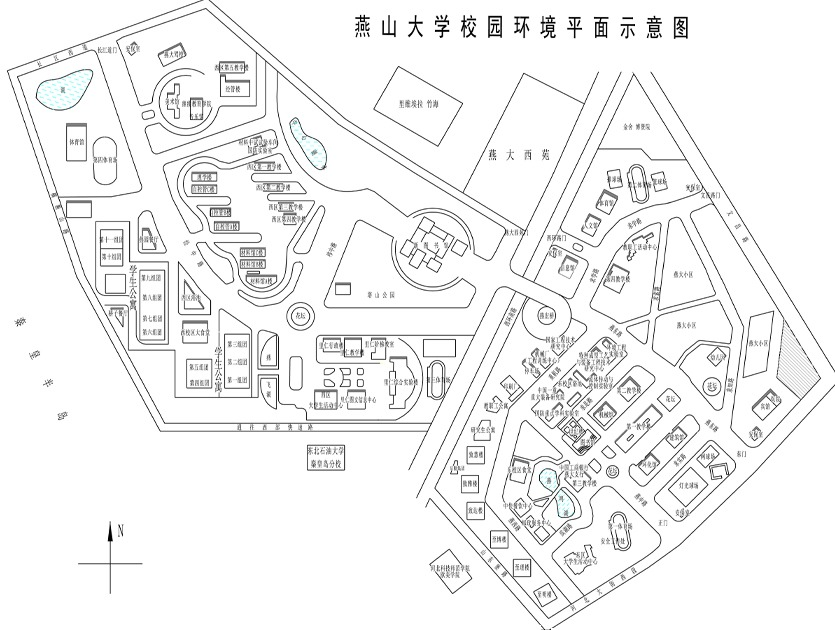
\includegraphics[width=0.95\textwidth]{figs/ysu_campus_map.jpg}
                    \caption{燕山大学校园导览图}
                    \label{fig1}
            \end{figure}
            
        \end{column}
    \end{columns}
\end{frame}

\subsection{脚注}

\begin{frame}
    \frametitle{脚注}
        可以在任何地方加入脚注，即便是在各种信息框\footnote{信息框包括：提示框、列表框、要点框等。}中也可以。
        \begin{notebox}[笔记]
            请大家把这里的笔记记录下来，是重点内容\footnote{考试要考。}。 
        \end{notebox}
\end{frame}

%最后一页
\makelast

\end{document}
